\newpage

\section{Problem 2 (14 pts)}

\subsection{Part 1}
\begin{enumerate}
\item Construct a formula in predicate logic to define a planet, where planet is defined
as an object whose mass is greater than $0.33 \times 10^{24}KG$, and which it orbits around the
sun. For all practical purposes, you may ignore the $10^{24}KG$ factor.\\

Formula for Planet:
\[\textit{Planet}(\textit{object}) \equiv \exists \textit{mass} \left( \textit{Mass}(\textit{object}, \textit{mass}) \land \textit{mass} > 0.33 \right) \land \textit{Orbits}(\textit{object}, \textit{sun})\]

Formula for \textit{is\_sattelite\_of}:
\[\textit{is\_sattelite\_of} \equiv \textit{Orbits}(\textit{sattelite}, \textit{object}) \land \textit{Planet}(\textit{object})\]
\\
\item Map your formulas to Prolog rules is planet/1, and is satellite of/2, and demonstrate how it works by executing both ground- and non-ground queries. Identify the type of each query.

Here we have the 2 main rules \textit{is\_planet} and
\textit{is\_satellite\_of}. 
    \begin{lstlisting}
    
        is_planet(P) :-
            object(P),
            mass(P, Mass),
            Mass >= 0.33,
            orbits(P, sun).

            
        is_satellite_of(S, P) :-
            object(S),
            is_planet(P),
            orbits(S, P).

            
    \end{lstlisting}

Below you can see the interaction with the Prolog interpreter(to be able to see the multiple results, you need to press \textit{space}).
    \begin{figure}[hbt!]
        \centering
        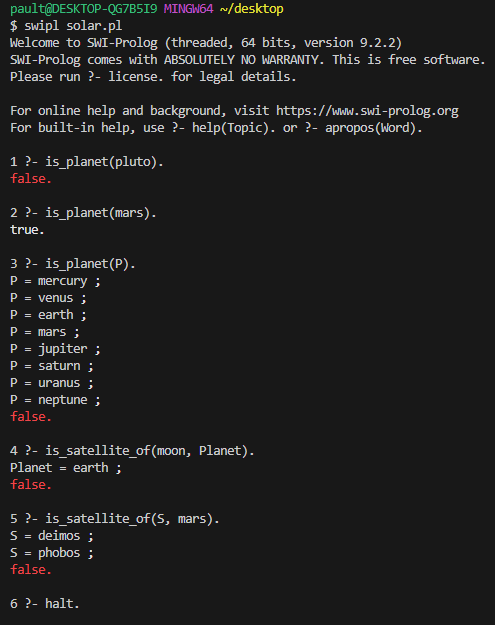
\includegraphics[scale=0.5]{assigment1/331A1_num2_part2.png}
        \caption{Prolog interaction for problem 2 part 2}
    \end{figure}\\
\newpage    
\item Construct a Prolog rule obtain all satellites/2 that succeeds by returning a collection of all satellites of a given planet.

Here we have the 2 main rules \textit{is\_planet} and \textit{is\_satellite\_of}.    
    \begin{lstlisting}
        is_planet(P) :-
            object(P),
            mass(P, Mass),
            Mass >= 0.33,
            orbits(P, sun).

        is_satellite_of(S, P) :-
            object(S),
            is_planet(P),
            orbits(S, P).
    \end{lstlisting}

    \begin{lstlisting}
        obtain_all_satellites(Planet, Satellites) :-
            findall(Satellite, is_satellite_of(Satellite, Planet)
            , Satellites).
    \end{lstlisting} \\
    \begin{figure}[hbt!]
        \centering
        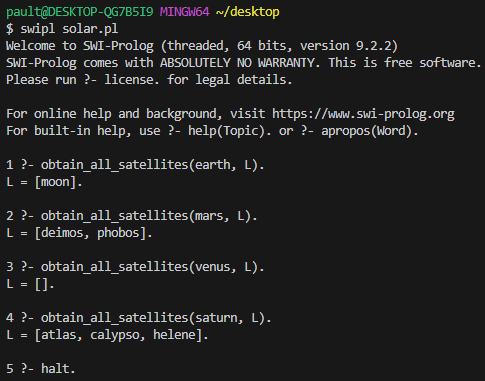
\includegraphics[scale=0.6]{assigment1/331A1_num2_part3.png}
        \caption{Prolog interaction for problem 2 part 3}
    \end{figure}\\

\end{enumerate}


\newpage

\subsection{Part 2: Categorical propositions}
\begin{enumerate}
    \item "Some numbers are not composite"\\
    \underline{Answer:}\\
    This is: $\exists x(number(x) \wedge \neg composite(x))$. Type  O.
    \\
    \item "No numbers are prime"\\
    \underline{Answer:}\\
    Rephrased as: "All numbers are composite". $\forall x(number(x) \wedge composite(x))$. Type A.
    \\
    \item "Some numbers are not prime"\\
    \underline{Answer:}\\
    Rephrased as: "Some numbers are composite". $\exists x(number(x) \wedge composite(x))$. Type I.
    \\
    \item "All numbers are prime"\\
    \underline{Answer:}\\
    Rephrased as: "No numbers are composite". $\forall x(number(x) \wedge \neg composite(x))$. Type E.
    \\
\end{enumerate}
\newpage
\subsection{Part 3: Categorical propositions}
\begin{enumerate}
    \item Prove formally that negating A is logically equivalent to obtaining O (and vice versa).\\ \\
Let A be the statement $\forall$ s : S \mid (s $\in$ P).\\
The negation of A, $\neg$A is $\neg(\forall$ s : S \mid (s $\in$ P)).\\
By De Morgan's, $\neg$A is equivalent to $\exists$ s : S \mid ($\neg$ (s $\in$ P)).\\
Therefore, negating A yields \textit{O}, since $\exists$ s : S \mid ($\neg$ (s $\in$ P)) is the definition of an \textit{O} proposition.

    \item Prove formally that negating E is logically equivalent to obtaining I (and vice versa).\\ \\
Let E be the statement $\neg(\exists$ s : S (s $\in$ P)).\\
The negation of E, $\neg$E is $\neg(\neg(\exists$ s : S (s $\in$ P))).\\
By the law of double negation, $\neg$E is equivalent to $\exists$ s : S (s $\in$ P).\\
Therefore, negating E yields \textit{I}, since $\exists$ s : S (s $\in$ P) is the definition of an \textit{I} proposition.


\end{enumerate}